\section{Design}
\label{sec:design}

\begin{figure}[t]
\centering
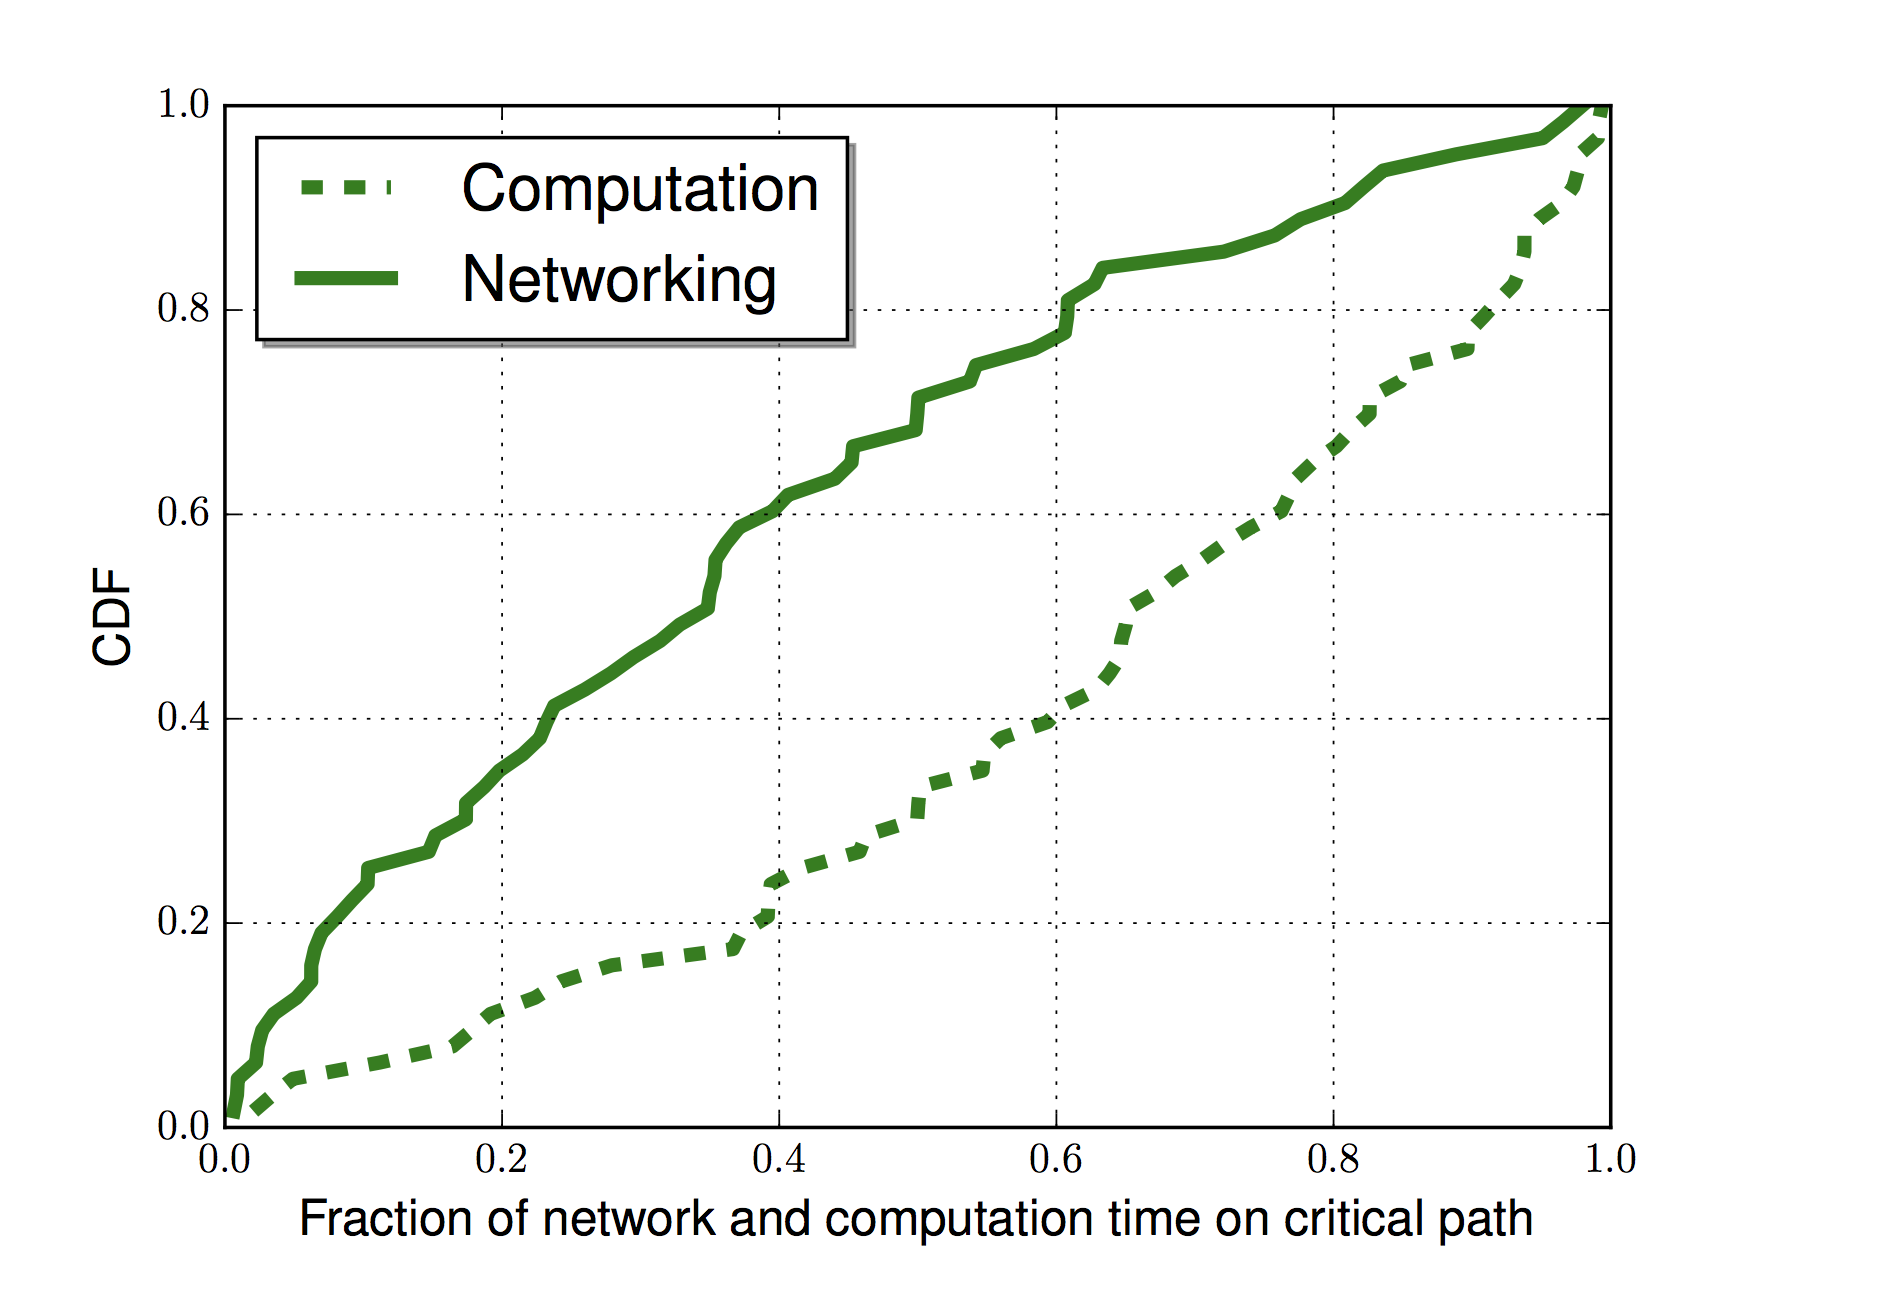
\includegraphics[width=0.9\columnwidth]{figs/comp_net.png}
\tightcaption{Runtime information on mobile devices}
\label{fig:mobile-runtime}
\end{figure}

\begin{figure}[t]
\centering
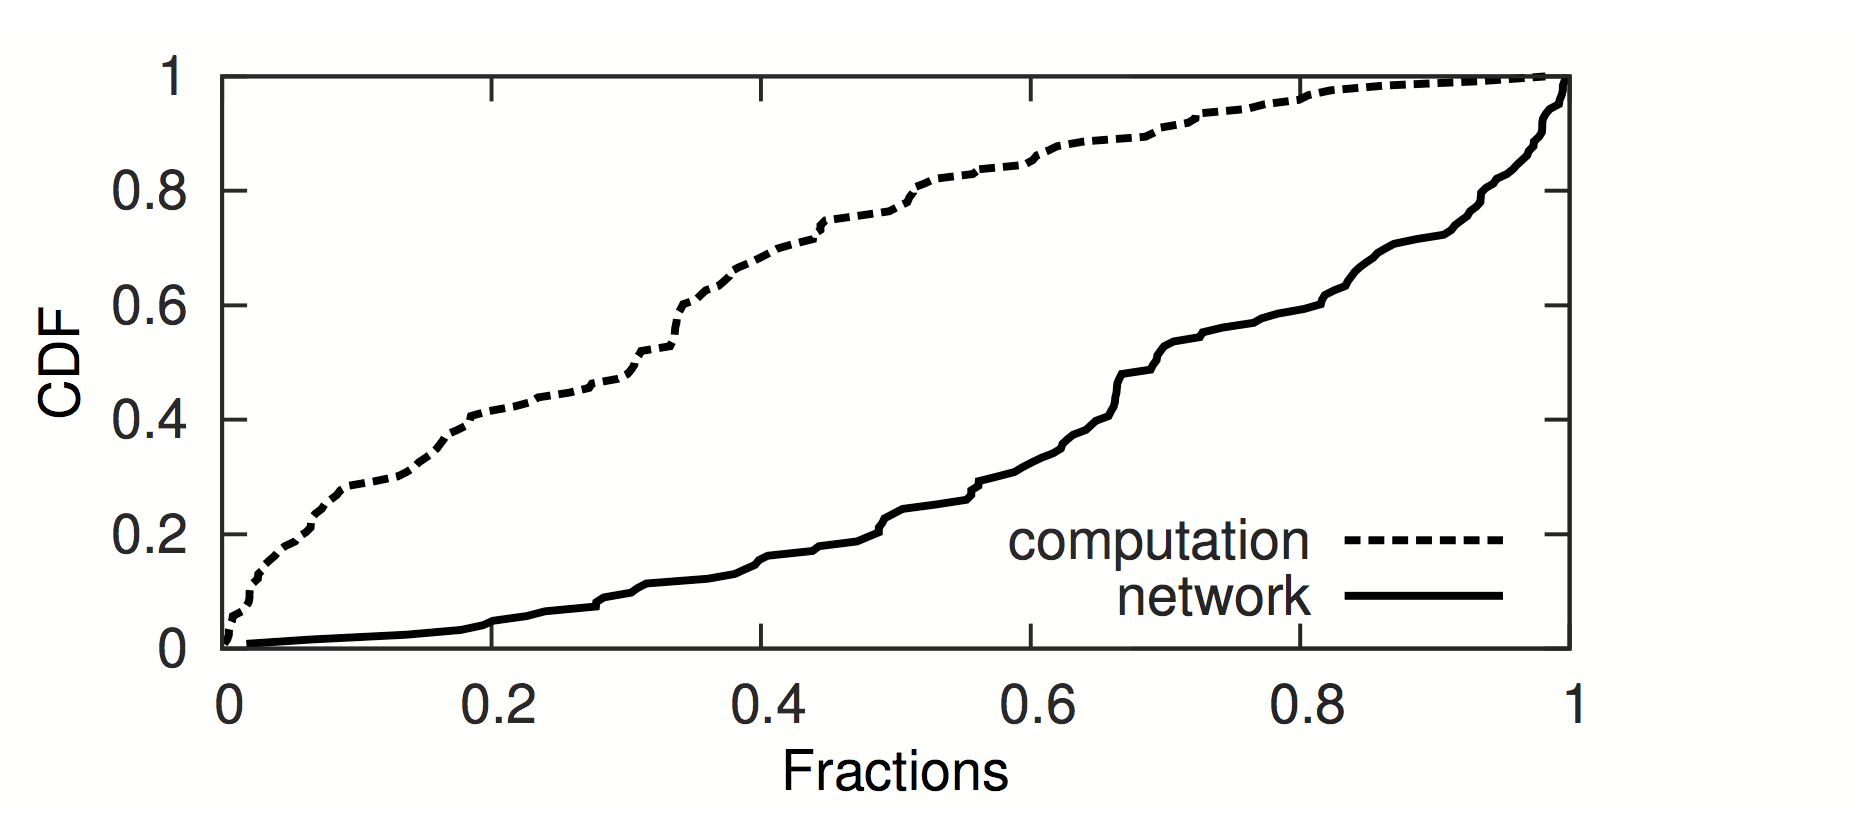
\includegraphics[width=0.9\columnwidth]{figs/comp_net_desk.png}
\tightcaption{Runtime information on desktops}
\label{fig:mobile-runtime}
\end{figure}

\begin{figure}[t]
\centering
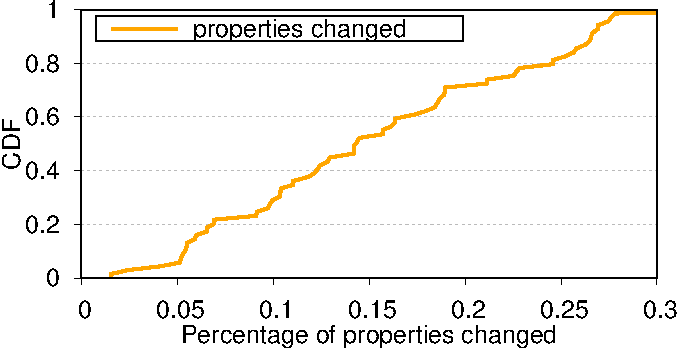
\includegraphics[width=0.9\columnwidth]{figs/cdf_bigdata_sec_new.pdf}
\tightcaption{Percentage of changed properties over 3 seconds}
\label{fig:properties-sec}
\end{figure}

\begin{figure}[t]
\centering
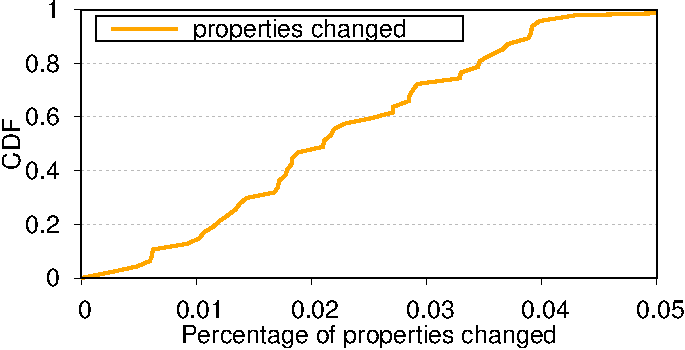
\includegraphics[width=0.9\columnwidth]{figs/cdf_bigdata_hr_new.pdf}
\tightcaption{Percentage of changed properties over 3 hours}
\label{fig:properties-hrs}
\end{figure}

\begin{figure}[t]
\centering
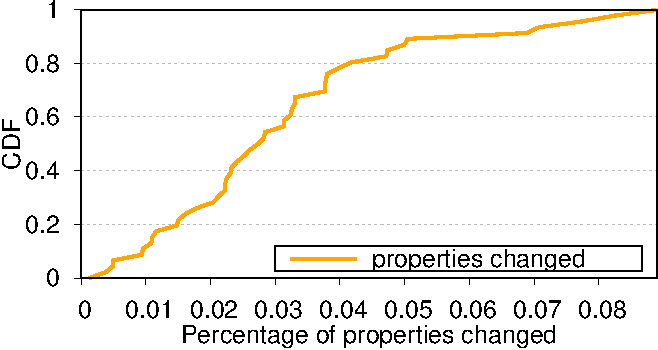
\includegraphics[width=0.9\columnwidth]{figs/cdf_bigdata_day_new.pdf}
\tightcaption{Percentage of changed properties over 3 days}
\label{fig:properties-day}
\end{figure}

% \begin{figure}[t]
% \centering
% \begin{tabular}{cc}
% 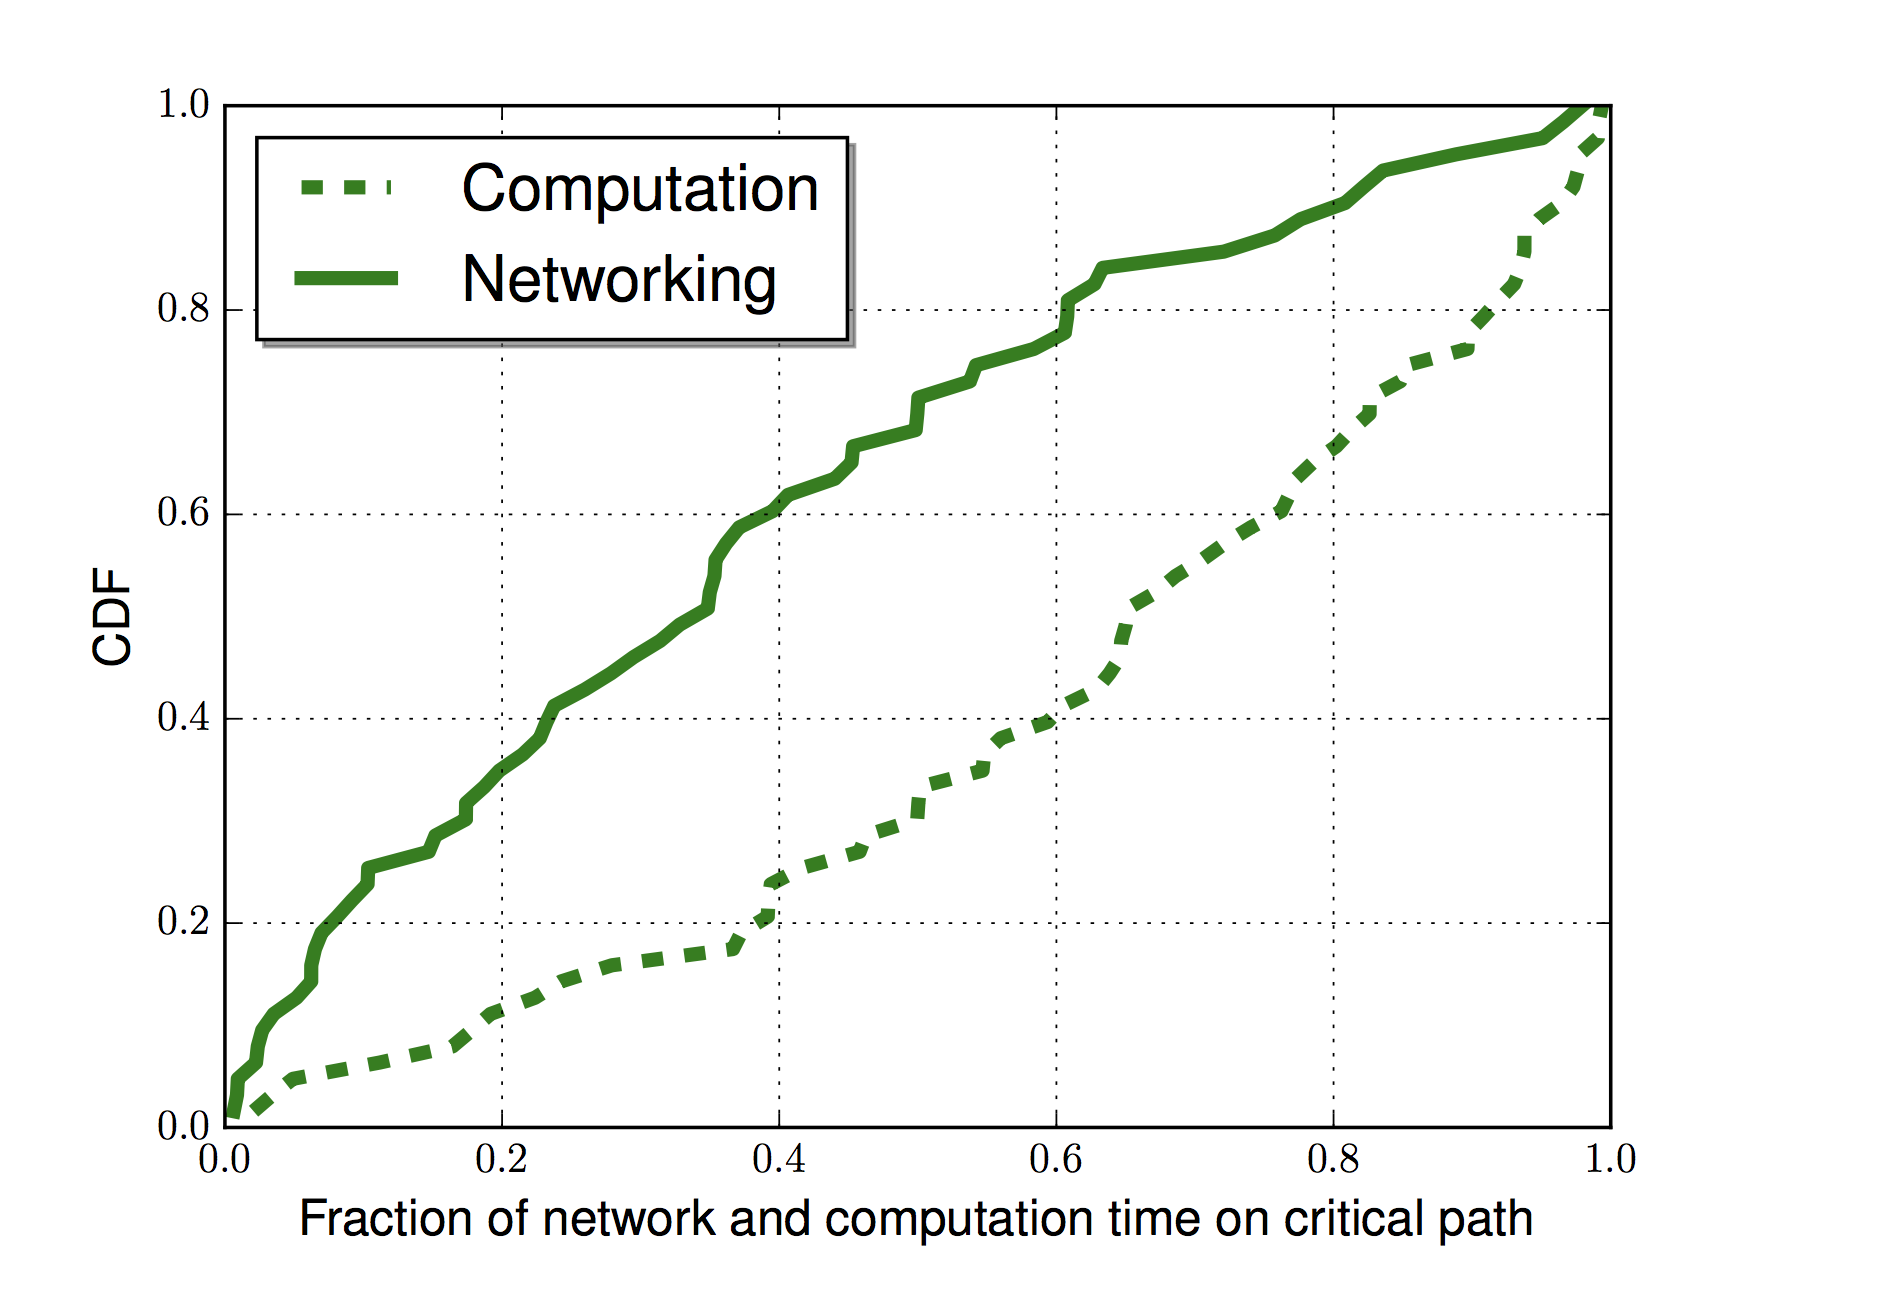
\includegraphics[width=0.9\columnwidth]{figs/comp_net.png}&
% 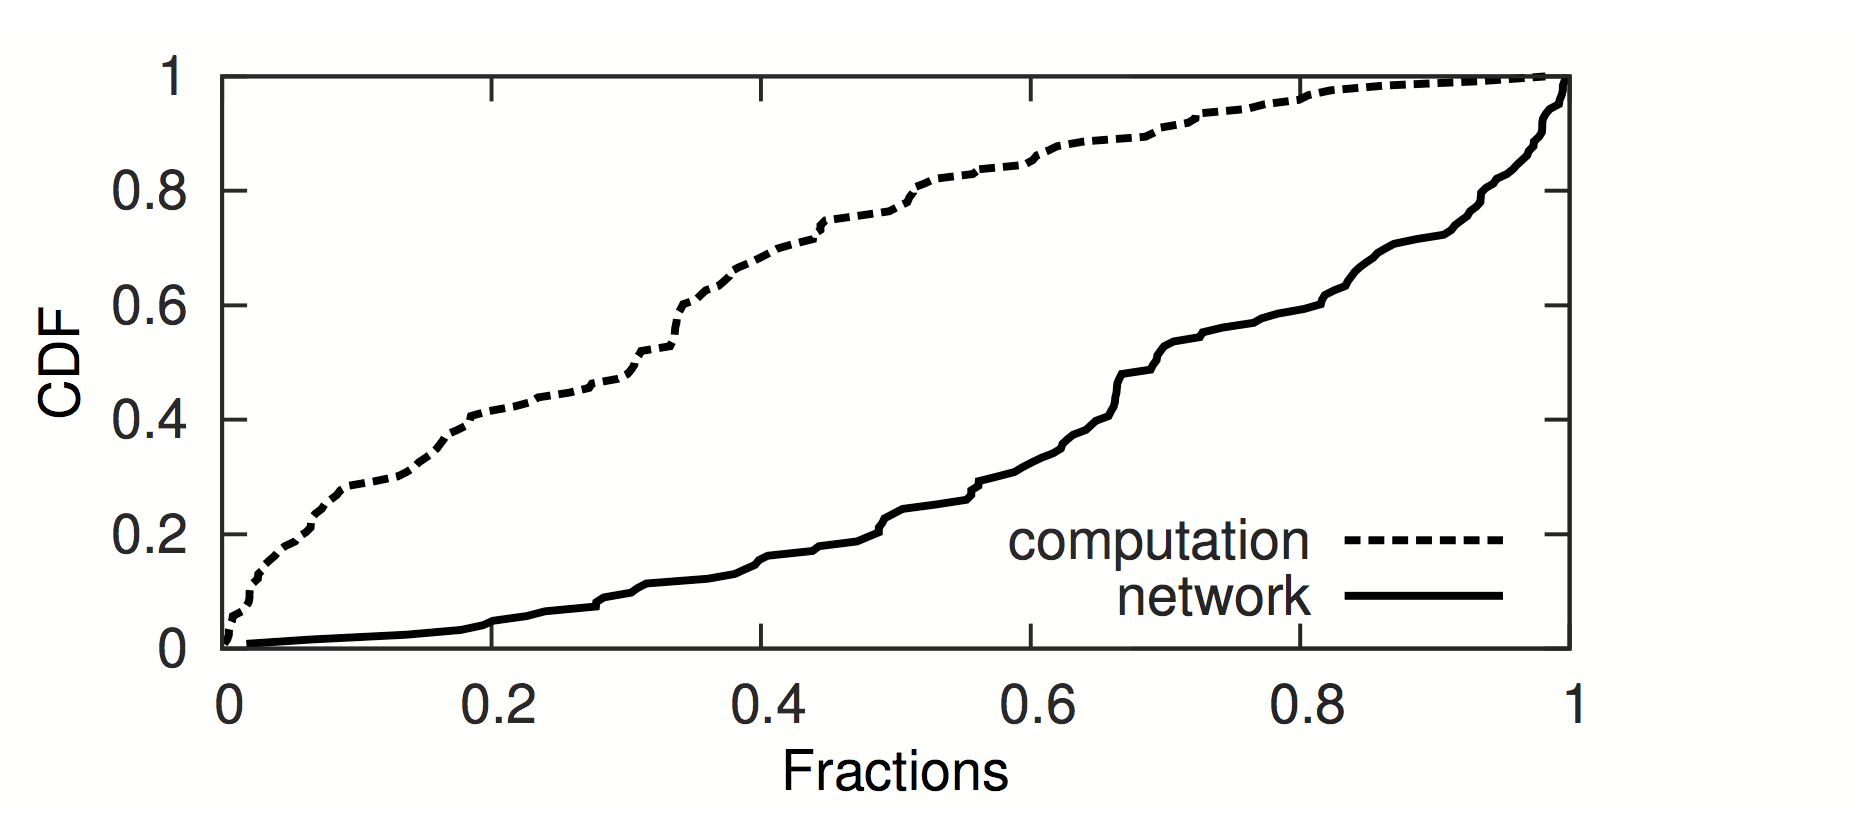
\includegraphics[width=0.9\columnwidth]{figs/comp_net_desk.png}\\
% {\small (a) Azure} & {\small (b) AWS}
% \end{tabular}
% \label{fig:dcs-local}
% \end{figure}

We propose a new technique to improve the page load time by reducing the javascript time,
specifically the execution and script evaluation time.  
In order to do this, we intend to build a new caching framework for the modern web browsers,
specifically Google Chrome. We choose to focus on Chrome because it accounts for about 50\% of the market share in terms of browser
usage. Our caching framework will store the javascript execution result. This can mean a lot of things
due to the dynamic nature of javascript. Most of the times it is simply the return value of the 
javascript functions. At other times it can be a modified DOM structure or just some intermediate result which
will be further processed by other javascript functions, later down the execution time line. 
We will talk about the exact definition of javascript execution output in section 3.1
The expiry of this javascript execution cache is supposed to be same as the expiry of the javascript source cache.
This essentially is derived from the x-cache header field in the response, which determines how long
the javascript source would reside in the browser cache. 
There are a lot of caveats to this approach, in the sense coming up with an optimal data structure to hold the 
javascript execution cache, handling non determinism of the javascript code, and in our work we will explore all of these.
The biggest challenge when developing a new caching framework is modifying the current browser's code 
in order to evaluate the efficacy of our caching framework. Since a lot of browsers already implement caching
at the javascript runtime level, such as compiler and parser caches, a lot of this architecture can be borrowed
for the execution cache as well. 
Another potential challenge will be the memory overhead. Most of the popular websites which spend about 70\% 
of their time on javascript execution are running 1000s of javascript functions. Saving the output of all 
of these functions will add extra memory overhead to current browsers. 

\subsection{Javascript Execution Output}
\label{sec:exec-output}

We have come up with a definition of the javascript execution output, which we will use in order
to build our caching framework. Currently we are working on two different granularities to 
capture the javascript execution output. The key idea behind capturing a javascript execution output 
is to capture the global changes made to the environment as a result of the javascript execution. 
This eliminates the need to capture any local computation, intermediate results computed and any output
in general which doesn't affect the global state of the browser. 
We define the global state of the browser to be represented by the window object, which is
an instance of the open window/tab of the browser. This window object is supported by all the 
major browsers like Chrome, Firefox, Safari. 
If the execution of any javascript doesn't modify the window object in any way, then essentially
that javascript has no affect to the global browser window state and therefore has null impact.
Such a javascript can be done away with, as long as any other global object which has used results
from this javascript's local computation was cached. This is the key idea behind our caching framework. 

The modification to the global window object can be either to the current properties of the window
object, which were modified by the javascript, or in form of creation of new properties. Any global variable
and function that is defined by the javascript becomes a new property of the window object.

The two granularities at which we'll capture the javascript execution output are:
\squishenum
\item Javascript file 
\item Javascript function
\squishenumend
The first point above is a higher granularity capture. To cater to this, we capture the entire window object state
before the page load begins, and after the page has been loaded. Then we do a basic diff analysis of these
two window states. This difference is essentially the global effects of that specific javascript. 
This helps us understand how much caching of the javascript execution output would ultimately impact the 
page loading time. 
To the best of our understanding, if 95\% properties of the global window object remain unchanged upon execution
of a particular javascript, then we have a theoretical upper bound of 95\% that we can achieve as far as reduction in 
javascript execution time is concerned, by employing our caching framework. We conducted a couple of experiments 
to understand how much change is made to the window object when the page is loaded after three seconds (Figure 3),
three hours (Figure 4) and three days (Figure 5). 
To our surprise, the change in the window object is extremely insignificant encouraging us to expect high impacts
of our caching framework. 

However javascript is rarely executed/evaluated as a file as a whole. Therefore to better understand the computation
effects of a javascript, we evaluate the execution output at the second granularity, at a function level. 
This will give us a much better understanding of the nature of the javascript execution, as javascript code is usually
invoked one function at a time. 
The approach here, is to create a call graph of the javascript execution, during a page load. Each node
in the graph represents a function that was actually invoked ( note that this a dynamic call graph, built
during the actual page load ). Each node contains a signature for the function that was executed. 
The signature contains the function name, arguments, any global variables declared, initialized or computed
and the return value. We use this signature to compare graphs across two different loads to 
establish how much of the execution can be cached. 


Caching of javascript execution is to be eventually implemented at a function level. The results from the above two studies
help us in defining the upper bound of the benefits of our approach. 
We are yet to implement the actual caching framework and evaluate the actual benefits of the approach.
